\chapter{Automatic Error Analysis} \label{chp:analysis}

\begin{center}
\textit{
  Preliminary versions of this chapter appeared as \textcite{Kummerfeld-etal:2012:EMNLP} and \textcite{Kummerfeld-etal:2013:ACL}.
}
\end{center}

Constituency parser performance is primarily interpreted through a single metric, F-score on \wsj section 23, that conveys no linguistic information regarding the remaining errors.
In this chapter, we describe a new error analysis method that classifies errors within a set of linguistically meaningful types using tree transformations that repair groups of errors together.
We use this analysis to answer a range of questions about parser behavior, including what linguistic constructions are difficult for state-of-the-art parsers, what types of errors are being resolved by rerankers, what types are introduced when parsing out-of-domain text, and how the challenges change for Chinese.

\begin{figure}
\begin{center}
\scalebox{\derivscale}{
\synttree
[S
	[NP
		[PRP [He]]]
	[VP
		[VBD [was]]
		[VP
			[VBN [named]]
			[\extranode{S}
				[\extranode{NP}
					[NP [.t chief executive officer]]
					[\extranode{PP}
						[IN [of]]
						[\extranode{NP}
							[NP
								[NNP [Applied]]]
							[PP [.t in 1986]]]]]]]]]
}

(a) Parser output
\vspace{3mm}

\scalebox{\derivscale}{
\synttree
[S
	[NP
		[PRP [He]]]
	[VP
		[VBD [was]]
		[VP
			[VBN [named]]
			[\missingnode{S}
				[\missingnode{NP}
					[NP [.t chief executive officer]]
					[\missingnode{PP}
						[IN [of]]
						[NP
							[NNP [Applied]]]]]]
			[PP [.t in 1986]]]]]
}

(b) Gold parse
\end{center}
\derivspace
\caption[Error analysis example: PP Attachment.]{ \label{fig:PP-attachment}
	\textbf{Incorrect PP~Attachment}, as \emph{(PP in~1986)} is too low.
	Bold, boxed nodes are either extra (marked in red in the parser output) or missing (marked in blue in the gold parse).
}
\derivaftercompress
\end{figure}

\section{Error Classification} \label{sec:errors-intro}

The standard metric for parsing is:

\begin{align*}
  \text{F}_1 & = \frac{2 * \text{precision} * \text{recall}}{\text{precision} + \text{recall}} \\
            & = \frac{2 * |\text{matching nodes}|}{|\text{nodes in gold parse}| + |\text{nodes in predicted parse}|}
\end{align*}

This is a robust metric that gives a sense of overall parser performance, but a single number cannot provide linguistically meaningful intuition for the source of remaining errors.
Since the metric is defined in terms of nodes, one natural direction for analysis is to break down the errors by node type.
Unfortunately, that approach is not particularly informative, as a single attachment error can cause multiple node errors, without a clear link between the two once aggregated.
For example, in Figure~\ref{fig:PP-attachment} there is a PP attachment error that causes seven bracket errors (extra S, NP, PP, and NP, missing S, NP, and PP).
Determining that these correspond to a PP attachment error from just the labels of the missing and extra nodes is difficult.
Additionally, once an aggregate count of node errors is made, different types of errors may contribute to the same count, for example mistakes in PP attachment and coordination could both contribute to the count of incorrect NP nodes.
In contrast, the approach we describe below takes into consideration the relations between node errors, grouping them into linguistically meaningful sets.

We classify node errors in two phases.
First, we find a set of tree transformations that convert the output parse into the gold parse (Section~\ref{sec:tree-transform}).
Second, each transformation is classified as one of several error types (Section~\ref{sec:classify}).
Pseudocode for our method is shown in Algorithm~\ref{alg:code}.
The tree transformation stage corresponds to the main loop, while the second stage corresponds to the final loop.

\begin{algorithm}[t]
\begin{algorithmic}
\State $U =$ initial set of node errors
\State Sort $U$ by the depth of the error in the parse, deepest first
\State $G = \emptyset$
\Repeat
	\ForAll{errors $e \in U$}
		\If{$e$ fits an environment template $t$}
			\State $g =$ new error group
			\State Correct $e$ as specified by $t$
			\ForAll{errors $f$ that $t$ corrects}
				\State Remove $f$ from $U$
				\State Insert $f$ into $g$
			\EndFor
			\State Add $g$ to $G$
		\EndIf
	\EndFor
\Until{unable to correct any further errors}
\ForAll{remaining errors $e \in U$}
	\State Insert a group into $G$ containing $e$
\EndFor
\ForAll{groups $g \in G$}
	\State Classify $g$ based on properties of the group
\EndFor
\end{algorithmic}
\caption{ \label{alg:code}
	Tree transformation error classification
}
\end{algorithm}

\subsection{Tree Transformations} \label{sec:tree-transform}

Our algorithm finds a path from the parser output to the gold parse, where states are parse structures and steps are transformations.
We define three general types of transformations:

\begin{description}
  \item[Create node] takes a set of nodes that are siblings and places them under a new node.
  \item[Delete node] removes a node and re-attaches its children where it was.
  \item[Move subtree] takes a node and moves it either up or down within the parse, with the constraint that it may not make the structure discontinuous. If this move leads to the creation of a unary production between two non-terminals of the same type, also remove one of them.
\end{description}

The first two of these are straightforward, while an example of the third can be seen in Figure~\ref{fig:PP-attachment}.
The PP node spanning \emph{in 1986} is moved up in the parse until it is outside of all the extra spans.
This fixes most of the errors, but leaves behind an NP to NP unary production.
One of the NPs is deleted, leaving behind the correct parse.

Once a transformation is performed, all of the nodes that were fixed are placed in a single group and information about the nearby parse structure before and after the transformation is recorded.
This recording is necessary, since subsequent changes may alter the surrounding structure in ways that impact the classification process described in the next section.

With this definition of states and transformations, a range of standard search algorithms are available to us.
We considered search algorithms with guarantees for finding the shortest path, but found they were prohibitively slow.
Instead, we find a path by applying a greedy bottom--up approach, iterating through the errors in the parse, deepest first.
Fortunately, on the shorter sentences for which finding the optimal path was feasible, we found that the greedy approach had no substantial impact on results.
This is the case because in many sentences a single correction will fix the parse and in cases with multiple errors they are often in disjoint sections of the parse.

\subsection{Transformation Classification} \label{sec:classify}

We began with a large set of node errors, in the first stage they were placed into groups, one group per tree transformation used to get from the automatically generated parse to the gold parse.
Now we classify each group as one of the error types below.
The ideal set of error classes would consider each group of incorrect constituents and show how their function has been misinterpreted by the parser, but it is difficult to define simple rules for such a classification.
In future work it would be interesting to build statistical models for classifying errors, using expert analysis of parse errors to train the system.
In the meantime, the approach we took was to construct general rules that classify errors mainly by the category of the nodes being moved and their surrounding context.
We developed our rules by running the system with no classification, then progressively adding rules to decrease the number of unclassified errors.
In the process of adding rules we also inspected observed classifications to check that they were correct, amending the rules if necessary.

\paragraph{PP Attachment} (Figure~\ref{fig:PP-attachment}) \\
Any case in which the transformation involved moving a Prepositional Phrase, or the incorrect bracket is over a PP, \myeg \\ 
\emph{He was} (VP \emph{named chief executive officer of} (NP \emph{Applied} (PP \emph{in 1986}))) \\
where (PP \emph{in 1986}) should modify the entire VP, rather than just \emph{Applied}.

\begin{figure}
\centering
\scalebox{\derivscale}{
\synttree
[NP
	[NP [.t A 16\% drop]]
	[\extranode{PP}
		[IN [for]]
		[\extranode{NP}
			[NP [.t Mannesmann AG]]
			[CC [and]]
			[NP [.t Dresdner AG's 10\% decline]]]]]
}

\vspace{3mm}
(a) Parser output

\vspace{6mm}

\scalebox{\derivscale}{
\synttree
[NP
	[\missingnode{NP}
		[NP [.t A 16\% drop]]
		[\missingnode{PP}
			[IN [for]]
			[NP [.t Mannesmann AG]]]]
	[CC [and]]
	[NP [.t Dresdner AG's 10\% decline]]]
}

\vspace{3mm}
(b) Gold parse
\derivspace
\caption[Error analysis example: Coordination.]{ \label{fig:coordination} 
	\textbf{Coordination} \emph{and Dresdner AG's 10\% decline} is too low.
}

\end{figure}

\paragraph{Coordination} (Figure~\ref{fig:coordination}) \\
Cases in which a conjunction is an immediate sibling of the nodes being moved, or is the leftmost or rightmost node being moved, \myeg \\
(NP \emph{A 16\% drop} (PP \emph{for} (NP (NP \emph{Mannesmann AG}) \emph{and} (NP \emph{Dresdner AG's 10\% decline})))) \\
where the conjunction and second NP should be at the top level, between \emph{A 16\% drop for Mannesmann AG} and \emph{Dresdner AG's 10\% decline}.

\paragraph{NP Attachment} (Figure~\ref{fig:NP-attachment}) \\
Several cases in which NPs had to be moved, particularly for mistakes in appositive constructions and incorrect attachments within a verb phrase, \myeg \\
\emph{The bonds} (VP \emph{go} (PP \emph{on sale} (NP \emph{Oct.\@\xspace 19}))) \\
where \emph{Oct.\@\xspace 19} should be an argument of \emph{go}.

\paragraph{Clause Attachment} (Figure~\ref{fig:clause-attachment}) \\
Any group that involves movement of some form of S node, \myeg \\
\emph{intends} (S (VP \emph{to} (VP \emph{restrict the RTC to ...\@\xspace} (SBAR \emph{unless the agency ...\@\xspace})))) \\
where the SBAR should be modifying \emph{intends}, rather than the lower VP.

\begin{landscape}
\begin{figure}
\centering
\begin{minipage}[b]{3.5in}
\centering
\scalebox{\derivscale}{
\synttree
[VP
	[VBD [wrote]]
		[\extranode{NP}
			[NP [.t another new ad]]
			[VBG [appearing]]]
		[NP
			[NN [today]]]]
}

\vspace{3mm}
(a) Parser output

\vspace{3mm}

\scalebox{\derivscale}{
\synttree
[VP
	[VBD [wrote]]
		[\missingnode{NP}
			[NP [.t another new ad]]
			[\missingnode{VP}
				[VBG [appearing]]
				[NP
					[NN [today]]]]]]
}

(b) Gold parse
\derivspace
\caption[Error analysis example: NP Attachment.]{ \label{fig:NP-attachment} 
	\textbf{NP Attachment}: \emph{today} is too high, it should be the argument of \emph{appearing}, rather than \emph{wrote}.
}

\end{minipage}\hfill
\begin{minipage}[b]{4.5in}
\centering
\scalebox{\derivscale}{
\synttree
[VP
	[VBZ [intends]]
	[\extranode{S}
		[\extranode{VP}
			[TO [to]]
			[\extranode{VP}
				[VB [restrict]]
				[NP [.t the RTC to \ldots]]
				[SBAR [.t unless the agency \ldots]]]]]]
}

\vspace{3mm}
(a) Parser output

\vspace{6mm}

\scalebox{\derivscale}{
\synttree
[VP
	[VBZ [intends]]
	[\missingnode{S}
		[\missingnode{VP}
			[TO [to]]
			[\missingnode{VP}
				[VB [restrict]]
				[NP [.t the RTC to \ldots]]]]]
	[SBAR [.t unless the agency \ldots]]]
}

\vspace{3mm}
(b) Gold parse
\derivspace
\caption[Error analysis example: Clause attachment.]{ \label{fig:clause-attachment} 
	\textbf{Clause Attachment} \emph{unless the agency receives specific congressional authorization} is attaching too low.
}

\end{minipage}
\end{figure}
\end{landscape}

\begin{figure}
\centering
\scalebox{\derivscale}{
\synttree
[NP
  [NP [.t federal financing]]
  [\extranode{PP}
    [IN [of]]
    [NP
      [NN [research]]]]
  [VP [.t using fetal tissue]]]
}

\vspace{3mm}
(a) Parser output

\vspace{6mm}

\scalebox{\derivscale}{
\synttree
[NP
  [NP [.t federal financing]]
  [\missingnode{PP}
    [IN [of]]
    [\missingnode{NP}
      [NP [NN [research]]]
      [VP [.t using fetal tissue]]]]]
}

\vspace{3mm}
(b) Gold parse
\derivspace
\caption[Error analysis example: VP attachment.]{ \label{fig:VP-attachment}
	\textbf{VP Attachment}: \emph{using fetal tissue} should modify \emph{research}, not \emph{financing}.
}

\end{figure}

\paragraph{VP Attachment} (Figure~\ref{fig:VP-attachment}) \\
When the correction involves moving a VP, \myeg \\
(NP (NP \emph{federal financing}) (PP \emph{of research}) (VP \emph{using fetal tissue})) \\
where the VP should modify \emph{research}, not \emph{financing}.

\paragraph{Adverb and Adjective Modifier Attachment} (Figure~\ref{fig:modifier-attachment}) \\
Cases involving incorrectly placed adjectives and adverbs, including errors corrected by subtree movement and errors requiring only creation of a node, \myeg \\
(NP (ADVP \emph{even more}) \emph{severe setbacks}) \\
where there should be an extra ADVP node over \emph{even more severe}.

\paragraph{Unary} (Figure~\ref{fig:unary}) \\
Mistakes involving unary productions that are not linked to a nearby error such as a matching extra or missing node, \myeg \\
(SINV (VP \emph{following}) \emph{is a breakdown of major market activity}) \\
where the VP should have an S above it.
In this particular example we can see how not modeling traces may be hurting performance--the S is intended to span both the VP and a null NP that is co-indexed with \emph{a breakdown of major market activity}.

\begin{landscape}
\begin{figure}
\centering
\begin{minipage}[b]{3in}
\scalebox{\derivscale}{
\synttree
[VP
	[VBD [had]]
	[\extranode{S}
		[\extranode{VP}
			[TO [to]]
			[\extranode{VP}
				[VB [think]]
				[PP [.t about it]]]]]
	[ADVP [.t ahead of time]]]
}

\vspace{3mm}
(a) Parser output

\vspace{6mm}

\scalebox{\derivscale}{
\synttree
[VP
	[VBD [had]]
	[\missingnode{S}
		[\missingnode{VP}
			[TO [to]]
			[\missingnode{VP}
				[VB [think]]
				[PP [.t about it]]
				[ADVP [.t ahead of time]]]]]]
}

\vspace{3mm}
(b) Gold parse
\derivspace
\caption[Error analysis example: Adverb and adjective modifier attachment.]{ \label{fig:modifier-attachment} 
	\textbf{Adverb and Adjective Modifier Attachment}: \emph{ahead of time} is too high, it should
	modify \emph{think}, not \emph{had}.
}

\end{minipage}\hfill
\begin{minipage}[b]{5in}
\centering
\scalebox{\derivscale}{
\synttree
[SINV
	[VP
		[VBG [Following]]]
	[VBZ [is]]
	[NP
		[NP [.t a breakdown]]
		[PP [.t of major market activity]]]]
}

\vspace{3mm}
(a) Parser output

\vspace{6mm}

\scalebox{\derivscale}{
\synttree
[SINV
	[\missingnode{S}
		[VP
			[VBG [Following]]]]
	[VBZ [is]]
	[\missingnode{NP}
		[NP
			[NP [.t a breakdown]]
			[PP [.t of major market activity]]]]]
}

\vspace{3mm}
(b) Gold parse

\vspace{6mm}

\scalebox{\derivscale}{
\synttree
[SINV
	[S-ADV
		[NP-SBJ
			[-NONE- [*-1]] ]
		[VP
			[VBG [Following]]]]
	[VBZ [is]]
	[NP-SBJ-1
		[NP
			[NP [.t a breakdown]]
			[PP [.t of major market activity]]]]]
}

\vspace{3mm}
(c) Gold parse with traces and function tags
\derivspace
\caption[Error analysis example: Unary.]{ \label{fig:unary} 
	Two \textbf{Unary} errors: a missing S and a missing NP.
	The third parse is the \ptb parse before traces and function tags are removed, included here to show the distinction between the two NPs in the production.
}

\end{minipage}
\end{figure}
\end{landscape}

\begin{figure}
\hfill
\begin{minipage}[b]{2.5in}
\centering
\scalebox{\derivscale}{
\synttree
[PP
	[IN [Unlike]]
	[\extranode{ADVP}
		[CD [two]]
		[NNS [years]]
		[RB [ago]]]]
}

\vspace{3mm}
(a) Parser output

\vspace{6mm}

\scalebox{\derivscale}{
\synttree
[PP
	[IN [Unlike]]
	[\missingnode{NP}
		[CD [two]]
		[NNS [years]]
		[RB [ago]]]]
}

\vspace{3mm}
(b) Gold parse
\derivspace
\caption[Error analysis example: Different label.]{ \label{fig:different-label}
	\textbf{Different Label}: \emph{two years ago} should be an NP.
}

\end{minipage}\hfill
\begin{minipage}[b]{3.5in}
\centering
\scalebox{\derivscale}{
\synttree
[NP
	[DT [a]]
	[\missingnode{ADJP}
	  [JJ [US-based]]]
	[NN [company]]]
}

\vspace{3mm}
(a) Missing node in parser output

\vspace{6mm}

\scalebox{\derivscale}{
\synttree
[PP
	[\extranode{ADVP}
	  [RB [Shortly]]]
	[IN [after]]
	[NP [.t 10 am]]]
}

\vspace{3mm}
(b) Extra node in parser output
\derivspace
\caption[Error analysis example: Single word phrase.]{ \label{fig:single-word-phrase}
	\textbf{Single Word Phrase}: Two examples, one in which the parser missed a node spanning a single word, and one in which it had an extra node.
}

\end{minipage}\hfill
\end{figure}

\paragraph{Different label} (Figure~\ref{fig:different-label}) \\
In many cases a node is present in the parse that spans the correct set of words, but has the wrong label, in which case we group the two node errors, (one extra, one missing), as a single error, \myeg \\
(PP \emph{Unlike} (ADVP \emph{two years ago})) \\
where the ADVP should be an NP.

\paragraph{Single word phrase} (Figure~\ref{fig:single-word-phrase}) \\
Node errors that span a single word, \myeg \\
(PP (ADVP \emph{Shortly}) \emph{after 10 a.m.\@\xspace}) \\
where the ADVP should not be present.
We include checks to ensure this is not linked to another error, such as one part of a set of internal noun phrase errors.

\paragraph{Parenthetical Attachment} (Figure~\ref{fig:PRN-attachment})
When a parenthetical node modifies at the wrong level, \myeg \\
(NP \emph{other forms} (PP \emph{of} (NP \emph{housing} (PRN \emph{(such as low-income)})))) \\
where the parenthetical should be higher.

\paragraph{Missing Parenthetical} (Figure~\ref{fig:missing-PRN})
When a parenthetical is entirely missing, \myeg \\
(S \emph{Moreover, explains one official, \ldots}) \\
where there should be a PRN around \emph{, explains one official,}.

\begin{landscape}
\begin{figure}
\begin{minipage}[b]{4in}
\centering
\scalebox{\derivscale}{
\synttree
[NP
  [NP [.t other forms]]
  [\extranode{PP} 
    [IN [of]]
    [\extranode{NP}
      [NP [NN [housing]]]
      [PRN [.t (such as low-income)]]]]]
}

\vspace{3mm}
(a) Parser output

\vspace{6mm}

\scalebox{\derivscale}{
\synttree
[NP
  [NP [.t other forms]]
  [\missingnode{PP} 
    [IN [of]]
    [NP [NN [housing]]]]
  [PRN [.t (such as low-income)]]]
}

\vspace{3mm}
(b) Gold parse
\derivspace
\caption[Error analysis example: Parenthetical attachment.]{ \label{fig:PRN-attachment}
	\textbf{Parenthetical Attachment}: the parenthetical should be higher.
}

\end{minipage}\hfill
\begin{minipage}[b]{4in}
\centering
\scalebox{\derivscale}{
\synttree
[S
  [ADVP [RB [Moreover]]]
  [,]
  [VP [VBZ [explains]]]
  [NP [.t one official]]
  [,]
  [\ldots]]
}

\vspace{3mm}
(a) Parser output

\vspace{6mm}

\scalebox{\derivscale}{
\synttree
[S
  [ADVP [RB [Moreover]]]
  [\missingnode{PRN}
    [\missingnode{SINV}
      [,]
      [VP [VBZ [explains]]]
      [NP [.t one official]]
      [,]]]
  [\ldots]]
}

\vspace{3mm}
(b) Gold parse
\derivspace
\caption[Error analysis example: Missing parenthetical.]{ \label{fig:missing-PRN}
	\textbf{Missing Parenthetical} \emph{, explains one official,} should be a parenthetical.
}

\end{minipage}
\end{figure}
\end{landscape}

\begin{figure}
\centering
\scalebox{\derivscale}{
\synttree
[PP
	[IN [Within]]
	[NP
    [IN [about]]
    [CD [siz]]
    [NNS [months]]]]
}

\vspace{3mm}
(a) Parser output

\vspace{6mm}

\scalebox{\derivscale}{
\synttree
[PP
	[IN [Within]]
	[NP
    [\missingnode{QP}
      [IN [about]]
      [CD [siz]]]
    [NNS [months]]]]
}

\vspace{3mm}
(b) Gold parse
\derivspace
\caption[Error analysis example: NP internal structure.]{ \label{fig:NP-internal-structure} 
	\textbf{NP Internal Structure} \emph{about six} should form a QP.
}

\end{figure}

\paragraph{NP Internal Structure} (Figure~\ref{fig:NP-internal-structure}) \\
While most NP structure is not annotated in the \ptb, there is some use of ADJP, NX, NAC and QP nodes.
We form a single group for each NP that has one or more errors involving these types of nodes, \myeg \\
(PP \emph{Within} (NP \emph{about six months})) \\
should have a QP over \emph{about six}.

\paragraph{Other}
There is a long tail of other errors.
Some could be placed within the categories above, but would require far more specific rules.

Working from only a raw list of node errors in a parse, it would be difficult to determine errors like those described above.
Even for error types that can be measured by counting node errors or rule production errors, our approach has the advantage that we identify groups of errors with a single cause.
For example, what appears as a missing unary production may correspond to an extra bracket that contains a subtree that attached incorrectly.
By grouping node errors and classifying each group as a single mistake, we are able to more precisely characterize the mistakes a parser makes.

\section{Results} \label{sec:errors-results}

We used sections 00 and 24 of the WSJ section of the \ptb as development data while constructing the tree transformation and error group classification methods.
All of our examples in text come from these sections as well, but for all tables of results we ran our system on section 23.
We chose to run our analysis on section 23 as it is the only section we are sure was not used in the development of any of the parsers, either for tuning or feature development.
Our evaluation is entirely focused on the errors of the parsers, so unless there is a particular construction that is unusually prevalent in section 23, we are not revealing any information about the test set that could bias future work.

Our evaluation is over a wide range of \ptb constituency parsers and their variants from the past twenty years.
For all parsers we used the publicly available version, with the standard parameter settings.

\begin{table}
\begin{center}
\begin{tabular}{|lccccr|}
	\hline
		System & P & R & F & Exact & Speed \\
	\hline
	\hline
		\multicolumn{6}{|c|}{Enhanced Training / Systems} \\
		Charniak S \& R (SR)       & 92.44 & 91.70 & 92.07 & 44.87 & 1.8 \\
		Charniak Re ranking (R)     & 91.78 & 91.04 & 91.41 & 44.04 & 1.8 \\
		Charniak Self-trained (S)  & 91.16 & 90.89 & 91.02 & 40.77 & 1.8 \\
	\hline
		\multicolumn{6}{|c|}{Standard Parsers} \\
		Berkeley                   & 90.30 & 89.81 & 90.06 & 36.59 & 4.2 \\
		Charniak                   & 89.88 & 89.55 & 89.71 & 37.25 & 1.8 \\
		SSN                        & 89.96 & 88.89 & 89.42 & 32.74 & 1.8 \\
		BUBS                       & 88.57 & 88.43 & 88.50 & 31.62 & 27.6 \\
		Bikel                      & 88.23 & 88.10 & 88.16 & 32.33 & 0.8 \\
		Collins-3                  & 87.82 & 87.50 & 87.66 & 32.22 & 2.0 \\
		Collins-2                  & 87.77 & 87.48 & 87.62 & 32.51 & 2.2 \\
		Collins-1                  & 87.29 & 86.90 & 87.09 & 30.35 & 3.3 \\
		Stanford Lexicalized (L)   & 86.35 & 86.49 & 86.42 & 27.65 & 0.7 \\
		Stanford Unlexicalized (U) & 86.48 & 85.09 & 85.78 & 28.35 & 2.7 \\
	\hline
\end{tabular}
\caption[\parseval results on \wsj section 23 for the parsers we consider.]{ \label{tab:standard-results} 
	\parseval results on \wsj section 23 for the parsers we consider.
  The columns are precision, recall, F-score, exact sentence match, and speed (sentences / sec).
  Coverage was left out as it was above 99.8\% for all parsers.
}
\end{center}
\end{table}

\paragraph{Berkeley} \parencite{Petrov-etal:2006,Petrov-Klein:2007}.
An unlexicalised parser with a grammar constructed with automatic state splitting.

\paragraph{\textcite{Bikel:2004}} implementation of \textcite{Collins:1997}.

\paragraph{BUBS} \parencite{Dunlop-Bodenstab-Roark:2011,Bodenstab-Dunlop-Hall-Roark:2011}.
A `grammar-agnostic constituent parser,' which uses a Berkeley Parser grammar, but parses with various pruning techniques to improve speed, at the cost of accuracy.

\paragraph{\textcite{Charniak:2000}}.
A generative parser with a maximum entropy-inspired model.
We also use the reranker \parencite{Charniak-Johnson:2005}, and the self-trained model \parencite{McClosky-Charniak-Johnson:2006}.

\paragraph{\textcite{Collins:1997}}.
A generative lexicalized parser, with three models, a base model, a model that uses subcategorisation frames for head words, and a model that takes into account traces.

\paragraph{SSN} \parencite{Henderson:2003,Henderson:2004}.
A statistical left-corner parser, with probabilities estimated by a neural network.

\paragraph{Stanford} \parencite{Klein-Manning:2003:ACL,Klein-Manning:2003:NIPS}.
We consider both the unlexicalised PCFG parser (-U) and the lexicalized factored parser (-L), which combines the PCFG parser with a lexicalized dependency parser.

Table~\ref{tab:standard-results} shows the standard performance metrics,
measured on section 23 of the \wsj, using all sentences.  Speeds were measured
using a Quad-Core Xeon CPU (2.33GHz 4MB L2 cache) with 16GB of RAM.
These results clearly show the variation in parsing performance, but they do
not show which constructions are the source of those variations.

\begin{table}
\begin{center}
\begin{tabular}{|lrrr|}
	\hline
		           &             & Nodes    &       \\
		Error Type & Occurrences & Involved & Ratio \\
	\hline
	\hline
		PP Attachment & 846 & 1455 & 1.7 \\
		Single Word Phrase & 490 & 490 & 1.0 \\
		Clause Attachment & 385 & 913 & 2.4 \\
		Adverb and Adjective Modifier Attachment & 383 & 599 & 1.6 \\
		Different Label & 377 & 754 & 2.0 \\
		Unary & 347 & 349 & 1.0 \\
		NP Attachment & 321 & 597 & 1.9 \\
		NP Internal Structure & 299 & 352 & 1.2 \\
		Coordination & 209 & 557 & 2.7 \\
		Unary Clause Label & 185 & 200 & 1.1 \\
		VP Attachment & 64 & 159 & 2.5 \\
		Parenthetical Attachment & 31 & 74 & 2.4 \\
		Missing Parenthetical & 12 & 17 & 1.4 \\
		Unclassified & 655 & 734 & 1.1 \\
	\hline
\end{tabular}
\caption[Breakdown of errors on section 23 for the Charniak parser with self-trained model and reranker.]{ \label{tab:charniak-breakdown}
	Breakdown of errors on section 23 for the Charniak parser with self-trained model and reranker.
	Errors are sorted by the number of times they occur.
	Ratio is the average number of node errors caused by each error we identify
	(\myie Nodes Involved / Occurrences).
}
\end{center}
\end{table}

Our system enables us to answer questions about parser behavior that could previously only be probed indirectly.
We demonstrate its usefulness by applying it to a range of parsers (here), to reranked K-best lists of various lengths, and to output for out-of-domain parsing (following sections).

First, in Table~\ref{tab:charniak-breakdown}, we focus on a detailed error breakdown for the best system we consider, the Charniak parser with a self-trained model and with reranking of the top fifty candidate parses produced by the parser \parencite{Charniak:2000,Charniak-Johnson:2005,McClosky-Charniak-Johnson:2006}.
For each of our error types, the table shows how many times it occurred in the 2,416 sentences in \wsj section 23 of the \ptb (Occurrences), the total number of nodes involved in the groups that were classified as each error type (Nodes Involved), and the ratio between the two (Nodes / Occurrences).

The ratios show that some errors typically cause only a single node error, where as others, such as coordination, generally cause several.
This means that considering counts of error groups would over-emphasize some error types, \myeg single word phrase errors are second most important by number of groups, but seventh by total number of node errors (not counting `Unclassified', which corresponds to many different errors).

In Table~\ref{tab:wsj23-comp} we consider the breakdown of parser errors on \wsj section 23.
The shaded area of each bar indicates the frequency of parse errors (\myie empty means fewest errors).
The area filled in is determined by the average number of node errors per sentence that are attributed to that type of error.
The average number of node errors per sentence for a completely full bar is indicated by the bottom row (Worst), and the value for a completely empty bar is indicated by the top row (Best).
We use counts of node errors to make the contributions of each error type to F-score more interpretable.

As expected, PP attachment is the largest contributor to errors, across all parsers.
Coordination is surprisingly low on the list (6th) given how significant the problem is considered in the community \parencite{N06-1020}.
This appears to indicate that parsers are better at coordination than at PP attachment, but the raw counts do not take into consideration the relative frequency of the two decisions.
We can get a sense of how frequent these decisions are by counting CCs and PPs in sections 02--21 of the treebank: 16,844 and 95,581 respectively.
These counts are only an indicator of the number of decisions as the nodes can be used in ways that do not involve a decision.
Taking into consideration the 6:1 ratio of decisions, the 4:1 ratio of errors is less surprising, and instead supports the belief that coordination scope ambiguity is very difficult.
However, it does appear that improvements in coordination accuracy will have a limited impact on our performance metrics.
One surprisingly common error involves unary productions.
Looking at the breakdown by unary type we found that clause labeling (S, SINV, etc) accounted for a large proportion of the errors.

\begin{landscape}
\begin{table*}
\setlength\fboxsep{0mm}
\setlength\fboxrule{0.05mm}
\begin{center}
\begin{tabular}{lccccccccccc}
	\hline
		&
		&
		PP &
		Clause &
		Diff &
		Mod &
		NP &
		&
		1-Word &
		&
		NP &
		\\
		Parser &
		F-score &
		Attach &
		Attach &
		Label &
		Attach &
		Attach &
		Co-ord &
		Span &
		Unary &
		\textcolor{white}{a}Int.\textcolor{white}{a} &
		Other \\
	\hline
	\hline
Best &  & 0.60 & 0.38 & 0.31 & 0.25 & 0.25 & 0.23 & 0.20 & 0.14 & 0.14 & 0.50 \\
Charniak-RS & 92.07 & \mybar{0.0} & \mybar{0.0} & \mybar{0.034042} & \mybar{0.0} & \mybar{0.0} & \mybar{0.0} & \mybar{0.0} & \mybar{0.0} & \mybar{0.0} & \mybar{0.0} \\
Charniak-R & 91.41 & \mybar{0.516546} & \mybar{1.397504} & \mybar{0.0} & \mybar{1.389222} & \mybar{0.85421} & \mybar{0.585366} & \mybar{0.69697} & \mybar{0.842106} & \mybar{0.64} & \mybar{1.045992} \\
Charniak-S & 91.02 & \mybar{0.8523} & \mybar{1.68271} & \mybar{0.885106} & \mybar{0.958084} & \mybar{1.330596} & \mybar{1.443902} & \mybar{0.969696} & \mybar{0.842106} & \mybar{2.855384} & \mybar{1.335086} \\
Berkeley & 90.06 & \mybar{2.692494} & \mybar{2.552584} & \mybar{1.361702} & \mybar{3.353294} & \mybar{2.184804} & \mybar{3.531708} & \mybar{1.863636} & \mybar{4.052632} & \mybar{1.624616} & \mybar{2.51774} \\
Charniak & 89.71 & \mybar{2.040356} & \mybar{4.292336} & \mybar{2.417022} & \mybar{4.598802} & \mybar{2.858316} & \mybar{3.570732} & \mybar{3.075758} & \mybar{1.342106} & \mybar{3.224616} & \mybar{2.47569} \\
SSN & 89.42 & \mybar{2.2728} & \mybar{1.868092} & \mybar{4.697872} & \mybar{5.772456} & \mybar{3.318276} & \mybar{3.960976} & \mybar{3.40909} & \mybar{3.31579} & \mybar{4.307692} & \mybar{2.68594} \\
BUBS & 88.63 & \mybar{4.687652} & \mybar{5.918004} & \mybar{4.051064} & \mybar{3.065868} & \mybar{3.12115} & \mybar{4.858536} & \mybar{3.818182} & \mybar{6.81579} & \mybar{2.28923} & \mybar{4.04205} \\
Bikel & 88.16 & \mybar{4.997578} & \mybar{3.522282} & \mybar{2.382978} & \mybar{5.461078} & \mybar{6.324436} & \mybar{7.55122} & \mybar{4.060606} & \mybar{4.789474} & \mybar{5.858462} & \mybar{4.331144} \\
Collins-3 & 87.66 & \mybar{5.294592} & \mybar{2.88057} & \mybar{5.514894} & \mybar{5.772456} & \mybar{6.045174} & \mybar{7.687804} & \mybar{5.19697} & \mybar{5.710526} & \mybar{7.31077} & \mybar{4.830486} \\
Collins-2 & 87.62 & \mybar{5.649718} & \mybar{2.980392} & \mybar{4.561702} & \mybar{5.94012} & \mybar{6.193018} & \mybar{8.0} & \mybar{5.212122} & \mybar{5.710526} & \mybar{7.40923} & \mybar{4.762156} \\
Collins-1 & 87.09 & \mybar{5.778854} & \mybar{4.00713} & \mybar{5.34468} & \mybar{6.754492} & \mybar{8.0} & \mybar{7.570732} & \mybar{6.0} & \mybar{6.0} & \mybar{8.0} & \mybar{5.392904} \\
Stanford-F & 86.42 & \mybar{5.753026} & \mybar{8.0} & \mybar{8.0} & \mybar{7.473054} & \mybar{7.195072} & \mybar{4.546342} & \mybar{8.0} & \mybar{6.236842} & \mybar{7.975384} & \mybar{6.806834} \\
Stanford-U & 85.78 & \mybar{8.0} & \mybar{7.94296} & \mybar{6.331914} & \mybar{8.0} & \mybar{6.899384} & \mybar{7.141464} & \mybar{6.818182} & \mybar{8.0} & \mybar{6.966154} & \mybar{8.0} \\
Worst &  & 1.12 & 0.61 & 0.51 & 0.39 & 0.45 & 0.40 & 0.42 & 0.27 & 0.27 & 1.13 \\
	\hline
\end{tabular}
	\caption[Average number of bracket errors per sentence due to the top ten error types.]{ \label{tab:wsj23-comp}
		Average number of bracket errors per sentence due to the top ten error types.
		For instance, Stanford-U produces output that has, on average,
		1.12 bracket errors per sentence that are due to PP attachment.  The scale
		for each column is indicated by the Best and Worst values.
	}
\end{center}
\end{table*}

\end{landscape}

By comparing the performance of the Collins parser with other systems we can see where performance has and has not changed over the past fifteen years.
There has been improvement across the board, but in some cases, \myeg clause attachment errors and different label errors, the change has been more limited (24\% and 29\% reductions respectively).
It is difficult to know why these ambiguities are more difficult, but three possibilities are:
(1) annotation errors may be more prevalent, making the potential for improvement vary,
(2) they pose fundamental difficulties for the community's overall approach to parsing,
(3) there may be biases in our automatic classification scheme.
We investigated the breakdown of the different label errors by label, but no particular cases of label confusion stand out, and we found that the most common cases remained the same between Collins and the top results.
Overall, it seems that these error types may have been unintentionally neglected in research and could be a productive area for future investigation.

It is also interesting to compare pairs of parsers that share aspects of their
architecture.  One such pair is the Stanford parser, where the factored parser
combines the unlexicalised parser with a lexicalized dependency parser.  The
main sources of the 0.64 gain in F-score are PP attachment and coordination.

Another interesting pair is the Berkeley parser and the BUBS parser, which uses
a Berkeley grammar, but improves speed by pruning.  The pruning methods used in
BUBS are particularly damaging for PP attachment errors and unary errors.

Various comparisons can be made between Charniak parser variants.  We discuss
the reranker below.  For the self-trained model
\textcite{McClosky-Charniak-Johnson:2006} performed some error analysis,
considering variations in F-score depending on the frequency of tags such as
PP, IN and CC in sentences.  Here we see gains on all error types, though
particularly for clause attachment, modifier attachment and coordination, which
fits with their observations.

\subsection{Reranking}

The standard dynamic programming approach to parsing limits the range of features that can be employed.
One way to deal with this issue is to modify the parser to produce the top $K$ parses, rather than just the 1-best, then use a model with more sophisticated features to choose the best parse from this list \parencite{collins:00}.
While re-ranking has led to gains in overall performance \parencite{Charniak-Johnson:2005}, there has been limited analysis of how effectively rerankers are using the list of parses they are ranking.
Recent work has explored this question in more depth, but focusing on how variation in inference and model parameters impacts performance on standard metrics \parencite{huang:08a,Ng-etal:2010,Auli-Lopez:2011,Ng-Curran:2012}.
We will explore the question from the perspective of observed errors, considering the potential for improvement using only the n-best list of parses, and how many errors a re-ranker actually avoids.

In Table~\ref{tab:reranking} we present a breakdown over error types for the
Charniak parser, using the self-trained model and reranker.  The oracle results
use the parse in each K-best list with the highest F-score.  While this may not
give the true oracle result, as F-score does not factor over sentences, it
gives a close approximation.  The table has the same columns as
Table~\ref{tab:wsj23-comp}, but the ranges on the bars now reflect the min and
max for these sets.

\begin{landscape}
\begin{table*}
\setlength\fboxsep{0mm}
\setlength\fboxrule{0.05mm}
\begin{center}
\begin{tabular}{lrccccccccccc}
	\hline
		&
		&
		&
		PP &
		Clause &
		Diff &
		Mod &
		NP &
		&
		1-Word &
		&
		NP &
		\\
		System &
		K &
		F-score &
		Attach &
		Attach &
		Label &
		Attach &
		Attach &
		Co-ord &
		Span &
		Unary &
		\textcolor{white}{a}Int.\textcolor{white}{a} &
		Other \\
	\hline
	\hline
\multicolumn{3}{l}{Best} & 0.08 & 0.04 & 0.08 & 0.05 & 0.06 & 0.04 & 0.08 & 0.04 & 0.04 & 0.11 \\
	\hline
& 1000 & 98.30 & \mybar{0.0} & \mybar{0.0} & \mybar{0.0} & \mybar{0.0} & \mybar{0.0} & \mybar{0.0} & \mybar{0.0} & \mybar{0.0} & \mybar{0.0} & \mybar{0.0} \\
& 100 & 97.54 & \mybar{0.669552} & \mybar{0.820734} & \mybar{1.386666} & \mybar{0.570328} & \mybar{0.91513} & \mybar{0.747664} & \mybar{1.21547} & \mybar{0.45946} & \mybar{1.149426} & \mybar{0.716822} \\
& 50 & 97.18 & \mybar{1.079366} & \mybar{1.028078} & \mybar{1.84} & \mybar{1.04817} & \mybar{1.490774} & \mybar{0.95701} & \mybar{1.723756} & \mybar{0.72973} & \mybar{1.586206} & \mybar{1.115808} \\
Oracle & 20 & 96.40 & \mybar{1.979798} & \mybar{2.056156} & \mybar{2.72} & \mybar{2.019268} & \mybar{2.568266} & \mybar{1.928972} & \mybar{2.519338} & \mybar{1.27027} & \mybar{2.16092} & \mybar{1.704142} \\
& 10 & 95.66 & \mybar{2.56277} & \mybar{2.902808} & \mybar{3.706666} & \mybar{2.728324} & \mybar{3.512916} & \mybar{2.751402} & \mybar{3.513812} & \mybar{2.18919} & \mybar{3.172414} & \mybar{2.49535} \\
& 5 & 94.61 & \mybar{3.62482} & \mybar{4.475162} & \mybar{4.773334} & \mybar{4.084778} & \mybar{4.708488} & \mybar{3.394392} & \mybar{4.685082} & \mybar{3.0} & \mybar{4.528736} & \mybar{3.584108} \\
& 2 & 92.59 & \mybar{5.737374} & \mybar{6.522678} & \mybar{7.066666} & \mybar{6.319846} & \mybar{6.509226} & \mybar{6.370094} & \mybar{6.38674} & \mybar{5.675676} & \mybar{6.643678} & \mybar{5.978022} \\
\hline
& 1000 & 92.07 & \mybar{7.243868} & \mybar{6.963282} & \mybar{7.466666} & \mybar{7.352602} & \mybar{7.232472} & \mybar{6.35514} & \mybar{6.585636} & \mybar{7.378378} & \mybar{5.310344} & \mybar{6.255284} \\
& 100 & 92.08 & \mybar{7.232324} & \mybar{7.075594} & \mybar{7.413334} & \mybar{7.368016} & \mybar{6.745388} & \mybar{6.53458} & \mybar{6.541436} & \mybar{7.351352} & \mybar{5.333334} & \mybar{6.262046} \\
& 50 & 92.07 & \mybar{7.238096} & \mybar{6.980562} & \mybar{7.333334} & \mybar{7.38343} & \mybar{6.804428} & \mybar{6.893458} & \mybar{6.585636} & \mybar{7.135136} & \mybar{5.333334} & \mybar{6.282334} \\
Charniak & 20 & 92.05 & \mybar{7.411256} & \mybar{6.686826} & \mybar{7.226666} & \mybar{7.583816} & \mybar{6.833948} & \mybar{6.57944} & \mybar{6.718232} & \mybar{7.216216} & \mybar{5.563218} & \mybar{6.343196} \\
& 10 & 92.16 & \mybar{7.111112} & \mybar{6.75594} & \mybar{7.466666} & \mybar{6.982658} & \mybar{6.804428} & \mybar{6.654206} & \mybar{6.607734} & \mybar{6.783784} & \mybar{5.931034} & \mybar{6.07946} \\
& 5 & 91.94 & \mybar{7.318904} & \mybar{7.023758} & \mybar{7.626666} & \mybar{7.522158} & \mybar{7.217712} & \mybar{6.57944} & \mybar{7.027624} & \mybar{6.45946} & \mybar{6.367816} & \mybar{6.27557} \\
& 2 & 91.56 & \mybar{7.457432} & \mybar{7.308856} & \mybar{7.84} & \mybar{7.7842} & \mybar{7.749078} & \mybar{7.581308} & \mybar{7.447514} & \mybar{7.324324} & \mybar{7.057472} & \mybar{6.870668} \\
& 1 & 91.02 & \mybar{8.0} & \mybar{8.0} & \mybar{8.0} & \mybar{8.0} & \mybar{8.0} & \mybar{8.0} & \mybar{8.0} & \mybar{8.0} & \mybar{8.0} & \mybar{8.0} \\
	\hline
		\multicolumn{3}{l}{Worst} & 0.66 & 0.43 & 0.33 & 0.26 & 0.28 & 0.26 & 0.23 & 0.16 & 0.19 & 0.60 \\
	\hline
\end{tabular}
	\caption[Average number of bracket errors per sentence for a range of K-best list lengths using the Charniak parser with reranking and the self-trained model.]{ \label{tab:reranking}
		Average number of bracket errors per sentence for a range of K-best list lengths using the Charniak parser with reranking and the self-trained model.
		The oracle results are determined by taking the parse in each K-best list with the highest F-score.
	}
\end{center}
\end{table*}
	

\end{landscape}

While there is improvement on all errors when using the reranker, there is very
little additional gain beyond the first 5-10 parses.  Even for the oracle
results, most of the improvement occurs within the first 5-10 parses.  The
limited utility of extra parses for the reranker may be due to the importance
of the base parser output probability feature (which, by definition, decreases
within the K-best list).
Another possibility is that there is less useful variation further down the K-best list.
The utility is higher for the oracle, but we do not see greater improvement further down the list because those parses will be combinations of a set of variations in the parse that change the model probability only slightly, rather than providing useful variation.

Interestingly, the oracle performance considerably improves across all error types, even at the 2-best level.
This indicates that the base parser model is not particularly biased against particular error types, as if it were we would expect that fixing it would require going further down the list of parses given as options.
Focusing on the rows for $K=2$ we
can also see two interesting outliers.  The PP attachment improvement of the
oracle is considerably higher than that of the reranker, particularly compared
to the differences for other errors, suggesting that the reranker lacks the
features necessary to make the decision better than the parser.  The other
interesting outlier is NP internal structure, which continues to make
improvements for longer lists, unlike the other error types.

\subsection{Out-of-Domain}

Parsing performance drops considerably when shifting outside of the domain a
parser was trained on \parencite{Gildea:2001}.
Previously, \textcite{Clegg:2005:EIT:1626315.1626317} evaluated parsers qualitatively on
node types and rule productions, while  \textcite{Bender:2011:PEO:2145432.2145479}
designed a Wikipedia test set to evaluate parsers on dependencies representing
ten specific linguistic phenomena.

To provide a deeper understanding of the errors arising when parsing outside of
the newswire domain, we analyze performance of the Charniak parser with
reranker and self-trained model on the eight parts of the Brown corpus
\parencite{ptb}, and two parts of the Google Web
corpus \parencite{Petrov:2012}.  Table~\ref{tab:domain-info} shows statistics for
the corpora.  The variation in average sentence lengths skew the results for
errors per sentence.  To handle this we divide by the number of words to
determine the results in Table~\ref{tab:charniak-domains}, rather than by the
number of sentences, as in previous figures.

There are several interesting features in the table.  First, on the Brown
datasets, while the general trend is towards worse performance on all errors,
NP internal structure is a notable exception and in some cases PP attachment
and unaries are as well.

In the other errors we see similar patterns across the corpora, except humor
(Brown R), on which the parser is particularly bad at coordination and clause
attachment.  This makes sense, as the colloquial nature of the text includes
more unusual uses of conjunctions, for example here \emph{no mistake} is a phrase that is unlikely to be in the \wsj, and if it were, would probably be preceded by a verb like \emph{make}:

\vspace{3mm}
\emph{She was a living doll and no mistake -- the ... }
\vspace{3mm}

\begin{landscape}
\begin{table*}
\setlength\fboxsep{0mm}
\setlength\fboxrule{0.05mm}
\begin{center}
\begin{tabular}{lccccccccccc}
	\hline
		&
		&
		PP &
		Clause &
		Diff &
		Mod &
		NP &
		&
		1-Word &
		&
		NP &
		\\
		Corpus &
		F-score &
		Attach &
		Attach &
		Label &
		Attach &
		Attach &
		Co-ord &
		Span &
		Unary &
		\textcolor{white}{a}Int.\textcolor{white}{a} &
		Other \\
	\hline
	\hline
Best &  & 0.022 & 0.016 & 0.013 & 0.011 & 0.011 & 0.010 & 0.009 & 0.006 & 0.005 & 0.021 \\
\wsj 23 & 92.07 & \mybar{1.440804} & \mybar{0.0} & \mybar{0.0} & \mybar{0.0} & \mybar{0.0} & \mybar{0.0} & \mybar{0.0} & \mybar{0.0} & \mybar{0.41602} & \mybar{0.0} \\
Brown-F & 85.91 & \mybar{4.896498} & \mybar{3.250554} & \mybar{1.631354} & \mybar{4.696056} & \mybar{1.598754} & \mybar{4.921258} & \mybar{1.995302} & \mybar{4.15448} & \mybar{0.647498} & \mybar{2.82369} \\
Brown-G & 84.56 & \mybar{5.508282} & \mybar{7.325484} & \mybar{1.853216} & \mybar{6.121282} & \mybar{2.78424} & \mybar{5.879576} & \mybar{1.938794} & \mybar{6.944538} & \mybar{0.897906} & \mybar{4.177172} \\
Brown-K & 84.09 & \mybar{2.778362} & \mybar{5.604532} & \mybar{3.375554} & \mybar{6.898596} & \mybar{2.502732} & \mybar{5.334422} & \mybar{3.016354} & \mybar{3.142288} & \mybar{0.516418} & \mybar{3.599498} \\
Brown-L & 83.95 & \mybar{2.053374} & \mybar{5.081866} & \mybar{3.647412} & \mybar{8.0} & \mybar{3.219792} & \mybar{3.006466} & \mybar{3.4229} & \mybar{2.052254} & \mybar{0.289788} & \mybar{3.919894} \\
Brown-M & 84.65 & \mybar{1.40727} & \mybar{3.807638} & \mybar{3.582916} & \mybar{4.179458} & \mybar{2.817122} & \mybar{2.846972} & \mybar{2.67492} & \mybar{0.66481} & \mybar{0.479804} & \mybar{3.184068} \\
Brown-N & 85.20 & \mybar{0.0} & \mybar{2.553112} & \mybar{3.58075} & \mybar{6.98768} & \mybar{2.352018} & \mybar{1.762212} & \mybar{3.036734} & \mybar{1.637836} & \mybar{0.0} & \mybar{2.869356} \\
Brown-P & 84.09 & \mybar{1.484664} & \mybar{5.614132} & \mybar{3.449038} & \mybar{7.527334} & \mybar{2.719566} & \mybar{6.024362} & \mybar{2.895496} & \mybar{3.982716} & \mybar{0.166918} & \mybar{4.164196} \\
Brown-R & 83.60 & \mybar{2.335016} & \mybar{8.0} & \mybar{2.692872} & \mybar{6.759088} & \mybar{2.954472} & \mybar{8.0} & \mybar{3.123632} & \mybar{5.673496} & \mybar{0.789784} & \mybar{4.470512} \\
G-Web Blogs & 84.15 & \mybar{8.0} & \mybar{5.920108} & \mybar{3.10226} & \mybar{7.195684} & \mybar{5.037776} & \mybar{5.845518} & \mybar{3.692442} & \mybar{4.424376} & \mybar{3.891982} & \mybar{7.804446} \\
G-Web Email & 81.18 & \mybar{6.204456} & \mybar{4.014904} & \mybar{8.0} & \mybar{3.42893} & \mybar{8.0} & \mybar{5.631512} & \mybar{8.0} & \mybar{8.0} & \mybar{8.0} & \mybar{8.0} \\
Worst &  & 0.040 & 0.035 & 0.053 & 0.020 & 0.034 & 0.023 & 0.046 & 0.009 & 0.029 & 0.073 \\
	\hline
\end{tabular}
	\caption{\label{tab:charniak-domains}
		Average number of node errors per word for a range of domains.
	}{
		Average number of node errors per word for a range of domains using the
		Charniak parser with reranking and the self-trained model.  We use per word
		error rates here rather than per sentence as there is great variation in
		average sentence length across the domains, skewing the per sentence
		results.
	}
\end{center}
\end{table*}
	

\end{landscape}

\begin{table}
\begin{center}
\begin{tabular}{|llrr|}
	\hline
		Corpus & Description & Sentences & Av. Length \\
	\hline
	\hline
		\wsj 23 & Newswire & 2416 & 23.5 \\
		Brown F & Popular & 3164 & 23.4 \\
		Brown G & Biographies & 3279 & 25.5 \\
		Brown K & General & 3881 & 17.2 \\
		Brown L & Mystery & 3714 & 15.7 \\
		Brown M & Science & 881 & 16.6 \\
		Brown N & Adventure & 4415 & 16.0 \\
		Brown P & Romance & 3942 & 17.4 \\
		Brown R & Humor & 967 & 22.7 \\
		G-Web Blogs & Blogs & 1016 & 23.6 \\
		G-Web Email & E-mail & 2450 & 11.9 \\
	\hline
\end{tabular}
\caption[Variation in size and contents of the domains we consider.]{ \label{tab:domain-info}
	Variation in size and contents of the domains we consider.	The variation in
	average sentence lengths skews the results for errors per sentences, and so
	in Table~\ref{tab:charniak-domains} we consider errors per word.
}
\end{center}
\end{table}

Comparing the Brown corpora and the Google Web corpora, there are much larger
divergences.  We see a particularly large decrease in NP internal structure.
Looking at some of the instances of this error, it appears to be largely caused
by incorrect handling of structures such as URLs and phone numbers, which do
not appear in the \ptb.  There are also some more difficult cases, for example:

\vspace{3mm}
\emph{... going up for sale in the next month or do .}
\vspace{3mm}

\noindent where \emph{or do} is a QP.
This typographical error of \emph{do} instead of \emph{two} is extremely difficult to handle for a parser trained only on well-formed text.

For e-mail there is a substantial drop on single word phrases.  Breaking the
errors down by label we found that the majority of the new errors are missing
or extra NPs over single words.  Here the main problem appears to be temporal
expressions, though there also appear to be a substantial number of errors that
are also at the POS level, such as when NNP is assigned to \emph{ta} in this
case:

\vspace{3mm}
\emph{... let you know that I 'm out ta here !}
\vspace{3mm}

Some of these issues, such as URL handling, could be resolved with suitable
training data.  Other issues, such as ungrammatical language and
unconventional use of words, pose a greater challenge.

%%%  ============================================================================
%%%  
%%%  This paper reports on the results of systematic analysis of errors
%%%  made by Chinese parsers.
%%%  
%%%  The experimental results are very interesting.
%%%  Though the basic methodology used in the paper builds directly
%%%  on a previous work, it is adapted well to Chinese through careful
%%%  analysis of error types.
%%%  
%%%  It would be nice to give more in-depth comparison with previous
%%%  findings on the difficulty of Chinese parsing, but I understand
%%%  the authors have already done well within the limited space.
%%%  
%%%  ============================================================================
%%%  
%%%  The paper is a thorough analysis of problems in Chinese parsing. I like it that
%%%  a variety of parsers were used. The paper is generally well written. The
%%%  results do not seem particularly surprising but it is good to have empirical
%%%  evidence to support them. The analysis and software should support future
%%%  research into the problematic areas.
%%%  However, I would suggest adding statistical significance tests, and reworking
%%%  Section 4. I understand that not all error categories can be discussed in
%%%  detail but the selection was unsatisfactory. Table 1 shows which error types
%%%  are new in this work, but not all of them are explained. It's not clear how the
%%%  order of subsections is determined. Some types are presented mostly to say that
%%%  they are less important than in English (PP attachment), while the second
%%%  biggest error type (coordination) is not discussed in this section at all, and
%%%  the third-highest only very briefly (not enough to make me understand why this
%%%  is substantially different from English).
%%%  Maybe for those categories that are comparable to Kummerfeld, you could add the
%%%  English percentages to Table 1?
%%%  I'm not so convinced by the final conclusion, NP internal structure is an issue
%%%  in English as well, just not in the PTB annotation. Coordination is still not
%%%  properly solved for English.
%%%  
%%%  ============================================================================
%%%  
%%%  This paper presents a comprehensive analysis of errors in Chinese Parsing,
%%%  and releases an open-source code for it.
%%%  
%%%  The author adapt the system from Kummerfeld et al.2012 to Chinese,
%%%  and examine a wide range of Chinese constitute Parsers.
%%%  Experimental results show a series of interesting findings,
%%%  mainly on verb-argument-attach-error and coordination errors.
%%%  The idea is clear and the paper is well written.
%%%  
%%%  What I miss is a more specific conclusion: I think it's not as deep as
%%%  Kummerfeld in 2012. Yes, empirically we can see the coord and verb args fields
%%%  are not quite improved even with gold POS tag. But I think it would be clearer
%%%  if the author can give some examples to explain why gold POS can't do that. And
%%%  this would help us to find the right direction to address these problems.

\section{Chinese Parsing}

Aspects of Chinese syntax result in a distinctive mix of parsing challenges.
However, the contribution of individual sources of error to overall difficulty is not well understood.  
We conduct a comprehensive automatic analysis of error types made by Chinese parsers, covering a broad range of error types for large sets of sentences, enabling the first empirical ranking of Chinese error types by their performance impact.  
To accommodate error classes that are absent in English, we augment the system to recognize Chinese-specific parse errors.
To understand the impact of part-of-speech tagging errors on different error types, we also performed a part-of-speech ablation experiment, in which particular confusions are introduced in isolation.
By analyzing the distribution of errors in the system output with and without gold part-of-speech tags, we are able to isolate and quantify the error types that can be resolved by improvements in POS tagging accuracy.
Our analysis shows that improvements in tagging accuracy can only address a subset of the challenges of Chinese syntax.
Further improvement in Chinese parsing performance will require research addressing other challenges, in particular, determining coordination scope.

\subsection{Background}

A decade of Chinese parsing research, enabled by the Penn Chinese Treebank \parencite[\pctb;][]{Xue:2005:NLE}, has seen Chinese parsing performance improve from 76.7 F$_1$ \parencite{Bikel-Chiang:2000:CLP} to 84.1 F$_1$ \parencite{Qian-Liu:2012:EMNLP}.
While recent advances have focused on understanding and reducing the errors that occur in segmentation and part-of-speech tagging \parencite{Qian-Liu:2012:EMNLP,Jiang-etal:2009:ACL,Forst-Fang:2009:EACL}, a range of substantial issues remain that are purely syntactic.

The closest previous work is the detailed manual analysis performed by \textcite{Levy-Manning:2003:ACL}.
While their focus was on issues faced by their factored PCFG parser \parencite{Klein-Manning:2003:NIPS}, the error types they identified are general issues presented by Chinese syntax in the \pctb.
They presented several Chinese error types that are rare or absent in English, including noun/verb ambiguity, NP-internal structure and coordination ambiguity due to \emph{pro}-drop.
They attributed some of these differences to treebank annotation decisions and others to meaningful differences in syntax, suggesting that closing the English-Chinese parsing gap demands techniques beyond those currently used for English.
Based on this analysis they considered how to modify their parser to capture the information necessary to model the syntax within the \pctb.
However, as noted in their final section, their manual analysis of parse errors in one hundred sentences only covered a portion of a single parser's output, limiting the conclusions they could reach regarding the distribution of errors in Chinese parsing.

\subsection{Adapting Error Analysis to Chinese} \label{sec:adapting_automatic_error_analysis_to_chinese}

Our analysis builds on the system described in Sections~\ref{sec:classify}~and~\ref{sec:tree-transform}, which finds the shortest path from the system output to the gold annotations, then classifies each transformation step into one of several error types.
When directly applied to Chinese parser output, the system placed over 27\% of the errors in the catch-all `Other' type.
Many of these errors clearly fall into one of a small set of error types, motivating an adaptation to Chinese syntax.

To adapt the system to Chinese, we developed a new version of the second stage of the system, which assigns an error category to each tree transformation step.

To characterize the errors the original system placed in the `Other' category,
we looked through one hundred sentences, identifying error types generated by
Chinese syntax that the existing system did not account for.
With these observations we were able to implement new rules to catch the
previously missed cases, leading to the set shown in Table~\ref{tab:errors}.
To ensure the accuracy of our classifications, we alternated between refining
the classification code and looking at affected classifications to identify
issues.  We also periodically changed the sentences from the development set
we manually checked, to avoid over-fitting.

Where necessary, we also expanded the information available during
classification.  For example, we use the structure of the final gold standard
parse when classifying errors that are a byproduct of sense disambiguation
errors.

\subsection{Chinese Parsing Errors} \label{sec:chinese_parsing_errors}

\begin{table}
\centering
\begin{tabular}{lrr}
  \hline
  Error Type & Brackets & \% of total \\
  \hline
  \hline
              NP-internal* & 6019 & 22.70\% \\
              Coordination & 2781 & 10.49\% \\
   Verb taking wrong args* & 2310 &  8.71\% \\
                     Unary & 2262 &  8.53\% \\
Adverb and Adjective Modifier Attachment & 1900 &  7.17\% \\
             One Word Span & 1560 &  5.88\% \\
           Different label & 1418 &  5.35\% \\
            Unary A-over-A & 1208 &  4.56\% \\
   Wrong sense/bad attachment* & 1018 &  3.84\% \\
      Noun boundary error* &  685 &  2.58\% \\
             VP Attachment &  626 &  2.36\% \\
         Clause Attachment &  542 &  2.04\% \\
             PP Attachment &  514 &  1.94\% \\
      Split Verb Compound* &  232 &  0.88\% \\
              Scope error* &  143 &  0.54\% \\
             NP Attachment &  109 &  0.41\% \\
                     Other & 3186 & 12.02\% \\
\hline
\end{tabular}
\caption[Breakdown of errors in Chinese parsing.]{ \label{tab:errors} 
  Errors made when parsing Chinese. Values are the number of bracket errors
  attributed to that error type. The values shown are for the Berkeley parser,
  evaluated on the development set. * indicates error types that were added or
  substantially changed as part of the adaptation to Chinese.
}
\end{table}

Table~\ref{tab:errors} presents the errors made by the Berkeley parser.
Below we describe the error types that are either new in this analysis, have had their definition altered, or have an interesting distribution.

In all of our results we follow the same approach as earlier, presenting the number of bracket errors (missing or extra) attributed to each error type.
As discussed in Section~\ref{sec:errors-results}, for the purpose of understanding the cause of the remaining performance gap, bracket counts are more informative than a direct count of each error type, because the impact on \parseval F-score varies between errors, \myeg a single attachment error can cause 20 bracket errors, while a unary error causes only one.

\begin{figure}
\begin{minipage}[b]{0.45\textwidth}
\centering
%%%\scalebox{1.2}{ 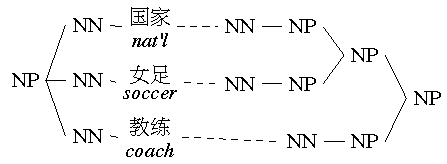
\includegraphics{figures/chinese-tree2} }

\begin{tikzpicture}
\tikzset{every tree node/.style={align=center}}
\Tree
[.NP 
  [.\extranode{NP}
    [.\extranode{NP} [.NN 国家\\national ] ]
    [.\extranode{NP} [.NN 女足\\soccer ] ] ]
  [.\extranode{NP} [.NN 教练\\coach ] ] ]
\end{tikzpicture}

\vspace{3mm}
(a) Parser output

\vspace{6mm}

\begin{tikzpicture}
\tikzset{every tree node/.style={align=center}}
\Tree
[.NP 
  [.NN 国家\\national ]
  [.NN 女足\\soccer ]
  [.NN 教练\\coach ] ]
\end{tikzpicture}

\vspace{3mm}
(b) Gold parse
\derivspace
\caption[Error analysis example: NP internal structure (Chinese).]{ \label{fig:np_internal} 
	\textbf{NP Internal Structure} This should be a flat structure.
}

\end{minipage}\hfill
\begin{minipage}[b]{0.5\textwidth}
\centering
%%%\scalebox{1.2}{ 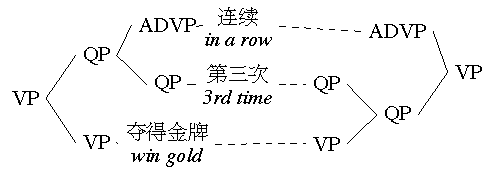
\includegraphics{figures/chinese-treemodatt} }

\begin{tikzpicture}
\tikzset{every tree node/.style={align=center}}
\Tree
[.VP
  [.ADVP 连续\\{in a row} ]
  [.\extranode{QP}
    [.QP 第三次\\{third time} ]
    [.VP 夺得金牌\\{win gold} ] ] ]
\end{tikzpicture}

\vspace{3mm}
(a) Parser output

\vspace{6mm}

\begin{tikzpicture}
\tikzset{every tree node/.style={align=center}}
\Tree
[.VP
  [.\missingnode{QP}
    [.ADVP 连续\\{in a row} ]
    [.QP 第三次\\{third time} ] ]
  [.VP 夺得金牌\\{win gold} ] ]
\end{tikzpicture}

\vspace{3mm}
(b) Gold parse
\derivspace
\caption[Error analysis example: Adverb and adjective modifier attachment (Chinese).]{ \label{fig:mod_att}
  \textbf{Modifier Attachment}: \glos{连续}{in a row} should modify only \glos{第三次}{third time}.
}

\end{minipage}
\end{figure}

\paragraph{NP-internal} (Figure~\ref{fig:np_internal}) \\
The \pctb annotates more NP-internal structure than the \ptb.
We assign this error type when a transformation involves words whose parts of speech in the gold parse are one of: CC, CD, DEG, ETC, JJ, NN, NR, NT and OD.

We investigated the errors that fall into the NP-internal category and found that 49\% of the errors involved the creation or deletion of a single pre-terminal phrasal bracket.
These errors arise when a parser proposes a parse in which POS tags (for instance, JJ or NN) occur as siblings of phrasal tags (such as NP), a configuration used by the PCTB bracketing guidelines to indicate complementation as opposed to adjunction \parencite{Xue:2005:NLE}.

\paragraph{Adverb and Adjective Modifier attachment} (Figure~\ref{fig:mod_att}) \\
Incorrect modifier scope caused by modifier phrase attachment level.
This is less frequent in Chinese than in English: while English VP modifiers occur in pre- and post-verbal positions, Chinese only allows pre-verbal modification.

\paragraph{Wrong sense/bad attachment} (Figure~\ref{fig:sense}) \\
This applies when the head word of a phrase receives the wrong POS, leading to an attachment error.
This error type is common in Chinese because of POS fluidity, \myeg the well-known Chinese verb/noun ambiguity often causes mis-attachments that are classified as this error type.

In Figure~\ref{fig:sense}, the word \mbox{\glos{投资}{invest}} has both noun and
verb senses. While the gold standard interpretation is the relative clause
\mbox{\Trans{firms that Macau invests in}}, the parser returned an NP
interpretation \mbox{\Trans{Macau investment firms}}.

\paragraph{Verb taking wrong args} (Figure~\ref{fig:wrong_arg}) \\
This error type
arises when a verb \mbox{(\myeg~\glos{扭转}{reverse})} is hypothesized to take
an incorrect argument (\mbox{\glos{布什}{Bush}} instead of
\mbox{\glos{地位}{position}}).  Note that this also covers some of the errors
that were classified as NP Attachment for English, changing
the distribution for that type.

\begin{figure}
\begin{minipage}[b]{0.45\textwidth}
\centering
%%%\scalebox{1.2}{ 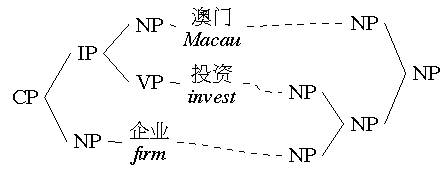
\includegraphics{figures/chinese-tree1} }

\begin{tikzpicture}
\tikzset{every tree node/.style={align=center}}
\Tree
[.\extranode{NP}
  [.NP 澳门\\Macau ]
  [.\extranode{NP}
    [.\extranode{NP} 投资\\invest ]
    [.NP 企业\\firm ] ] ]
\end{tikzpicture}

\vspace{3mm}
(a) Parser output

\vspace{6mm}

\begin{tikzpicture}
\tikzset{every tree node/.style={align=center}}
\Tree
[.\missingnode{CP}
  [.\missingnode{IP}
    [.NP 澳门\\Macau ]
    [.\missingnode{VP} 投资\\invest ] ]
  [.NP 企业\\firm ] ]
\end{tikzpicture}

\vspace{3mm}
(b) Gold parse
\derivspace
\caption[Error analysis example: Word sense confusion (Chinese).]{ \label{fig:sense} 
  \textbf{Sense Confusion} By treating \glos{投资}{invest} as a noun, the parser forms an NP about a type of firm, rather than a clause about action by \Trans{Macau}.
}

\end{minipage}\hfill
\begin{minipage}[b]{0.5\textwidth}
\centering
%%%\scalebox{1.2}{ 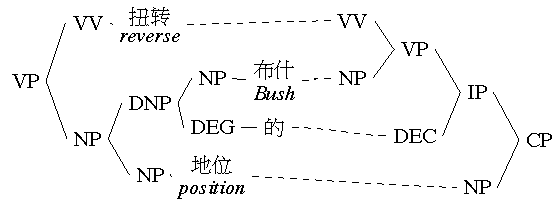
\includegraphics{figures/chinese-treebush} }

\begin{tikzpicture}
\tikzset{every tree node/.style={align=center}}
\Tree
[.\extranode{CP}
  [.\extranode{IP}
    [.\extranode{VP}
      [.VV 扭转\\reverse ]
      [.NP 布什\\Bush ] ]
    [.\extranode{DEC} 的 ] ]
  [.NP 地位\\position ] ]
\end{tikzpicture}

\vspace{3mm}
(a) Parser output

\vspace{6mm}

\begin{tikzpicture}
\tikzset{every tree node/.style={align=center}}
\Tree
[.\missingnode{VP}
  [.VV 扭转\\reverse ]
  [.\missingnode{NP}
    [.\missingnode{DNP}
      [.NP 布什\\Bush ]
      [.\missingnode{DEG} 的 ] ]
    [.NP 地位\\position ] ] ]
\end{tikzpicture}

\vspace{3mm}
(b) Gold parse
\derivspace

\caption[Error analysis example: Verb taking wrong arguments (Chinese).]{ \label{fig:wrong_arg}
  \textbf{Verb Taking Wrong Arguments}: the verb takes the argument \glos{布什}{Bush} too early, before it has been bound with \glos{地位}{position}.
}

\end{minipage}
\end{figure}

\paragraph{Unary} \strut \\
For mis-application of unary rules we separate out instances in which the two brackets in the production have the the same label (A-over-A).
This case is created when traces are eliminated, a standard step in evaluation.
More than a third of unary errors made by the Berkeley parser are of the A-over-A type.
This can be attributed to two factors: (i) the \pctb annotates non-local dependencies using traces, and (ii) Chinese syntax generates more traces than English syntax, such as \emph{pro}-drop, the omission of arguments where the referent is recoverable from discourse \parencite{Guo-Wang-VanGenabith:2007:EMNLP}.
However, for parsers that do not return traces they are a benign error.

\paragraph{Noun boundary error} \strut \\
In this error type, a span is moved to a
position where the POS tags of its new siblings all belong to the
list of NP-internal structure tags which we identified above, reflecting
the inclusion of additional material into an NP.

\paragraph{Split verb compound} \strut \\
The \pctb annotations recognize several
Chinese verb compounding strategies, such as the serial verb construction
(\mbox{\glos{规划建设}{plan [and] build}}) and the resultative construction
(\mbox{\glos{煮熟}{cook [until] done}}), which join a bare verb to another
lexical item.  We introduce an error type specific to Chinese, in which such
verb compounds are split, with the two halves of the compound placed in
different phrases.

\paragraph{Scope error} \strut \\
These are cases in which a new span must be added to more closely bind a modifier phrase (ADVP, ADJP, and PP), for example, in 
(IP (ADVP \mbox{\glos{仅}{Only}}) (NP \mbox{\glos{去年}{last year,}}) (NP \mbox{\glos{中国 银行}{Bank of China}}) \ldots), the ADVP should modify the first NP only, which can be indicated by adding an NP to form (NP (ADVP \mbox{\glos{仅}{Only}}) (NP \mbox{\glos{去年}{last year}})).

\paragraph{PP attachment} \strut \\
This error type is rare in Chinese, as adjunct PPs are pre-verbal.  It does
occur near coordinated VPs, where ambiguity arises about which of the conjuncts
the PP has scope over.  Whether this particular case is PP attachment or
coordination is debatable; we follow the approach above and
label it PP attachment.

\subsection{Chinese-English Comparison} \label{subsec:chinese_english_comparison}

It is difficult to directly compare error analysis results for Chinese and
English parsing because of substantial changes in the classification method,
and differences in treebank annotations.

As described in the previous section, the set of error categories considered for Chinese is very different to the set of categories for English.  
Even for some of the categories that were not substantially changed, errors may be classified differently because of cross-over between two categories (\myeg between Verb taking wrong args and NP Attachment).

Differences in treebank annotations also present a challenge for cross-language error comparison.
The most common error type in Chinese, NP-internal structure, is rare in the English results, but the datasets are not comparable because the \ptb has much more limited NP-internal structure annotated than the \pctb.
Further characterization of the impact of annotation differences on errors is beyond the scope of this work.

Three conclusions that can be made are that (i) coordination is a more common issue in Chinese, but remains difficult in
both languages, (ii) PP attachment is a much greater problem in English, and
(iii) substantial challenges are posed by the higher frequency of
syntactic structures generating traces and null-elements in Chinese compared to English.

\subsection{Cross-Parser Analysis} \label{sec:cross_parser_analysis}

The previous section described the error types and their distribution for a single Chinese parser.
Here we confirm that these are general trends, by showing that the same pattern
is observed for several different parsers on the \pctb 6 dev set.\footnote{
  We use the standard data split suggested by the \pctb 6 file manifest.
  As a result, our results differ from those previously reported on other splits.
}
We include results for
a transition-based parser \parencite[ZPAR;][]{Zhang-Clark:2009:ICPT},
a split-merge PCFG parser \parencite{Petrov-etal:2006,Petrov-Klein:2007,Petrov:2010:NAACLHLT},
a lexicalized parser \parencite{Bikel-Chiang:2000:CLP},
and a factored PCFG and dependency parser
\parencite{Levy-Manning:2003:ACL,Klein-Manning:2003:ACL,Klein-Manning:2003:NIPS}.
\footnote{These parsers represent a variety of parsing methods, though exclude
some recently developed parsers that are not publicly
available \parencite{Qian-Liu:2012:EMNLP,Xiong-etal:2005:IJCNLP}.}

Comparing the two Stanford parsers in Table~\ref{tab:comparison}, the factored
model provides clear improvements on sense disambiguation, but performs
slightly worse on coordination.

The Berkeley product parser we include uses only two grammars because we found,
in contrast to the English results \parencite{Petrov:2010:NAACLHLT}, that further
grammars provided limited benefits.  Comparing the performance with the
standard Berkeley parser it seems that the diversity in the grammars only
assists certain error types, with most of the improvement occurring in four of
the categories, while there is no improvement, or a slight decrease, in five categories.

\begin{landscape}
\begin{table*}
\centering
\setlength\fboxsep{0mm}
\setlength\fboxrule{0.05mm}
\begin{tabular}{|lccccccccccccc|}
	\hline
	    & NP &  & Verb &  & Mod. & 1-Word & Diff & Wrong & Noun & VP & Clause & PP & \\
	System \hfill F$_1$ & Int. & Coord & Args & Unary & Attach & Span & Label & Sense & Edge & Attach & Attach & Attach & Other \\
	\hline
	\hline
	\emph{Best}    & 1.54 & 1.25 & 1.01 & 0.76 & 0.72 & 0.21 & 0.30 & 0.05 & 0.21 & 0.26 & 0.22 & 0.18 & 1.87 \\
	Berk-G$\;$ \hfill 86.8 &  \mybar{3.117775} &  \mybar{5.719997} &  \mybar{4.868075} &  \mybar{4.092204} &  \mybar{3.414187} &  \mybar{1.560478} &  \mybar{2.304226} &  \mybar{0.417061} &  \mybar{3.003337} &  \mybar{4.124765} &  \mybar{4.199998} &  \mybar{3.250795} &  \mybar{3.627305} \\
	Berk-2 \hfill 81.8 &  \mybar{5.106060} &  \mybar{5.726296} &  \mybar{4.657457} &  \mybar{5.602480} &  \mybar{3.889412} &  \mybar{5.874318} &  \mybar{5.465338} &  \mybar{4.259078} &  \mybar{4.180596} &  \mybar{4.645864} &  \mybar{3.974996} &  \mybar{4.055024} &  \mybar{4.120634} \\
	Berk-1 \hfill 81.1 &  \mybar{5.637080} &  \mybar{5.854733} &  \mybar{4.914895} &  \mybar{5.637384} &  \mybar{4.160972} &  \mybar{5.409644} &  \mybar{5.105299} &  \mybar{4.288569} &  \mybar{4.581930} &  \mybar{4.594485} &  \mybar{4.516671} &  \mybar{4.351321} &  \mybar{4.375378} \\
	ZPAR \hfill 78.1 &  \mybar{5.603375} &  \mybar{6.374733} &  \mybar{5.487246} &  \mybar{7.386910} &  \mybar{5.851629} &  \mybar{5.863920} &  \mybar{6.833466} &  \mybar{4.423375} &  \mybar{5.725748} &  \mybar{5.299080} &  \mybar{6.791682} &  \mybar{6.653960} &  \mybar{5.833838} \\
	Bikel \hfill 76.1 &  \mybar{6.464990} &  \mybar{7.357862} &  \mybar{6.227640} &  \mybar{6.372585} &  \mybar{6.280885} &  \mybar{6.602543} &  \mybar{5.609351} &  \mybar{6.904680} &  \mybar{8.000000} &  \mybar{5.790822} &  \mybar{6.700012} &  \mybar{6.484650} &  \mybar{5.983631} \\
	Stan-F \hfill 76.0 &  \mybar{6.824621} &  \mybar{8.000000} &  \mybar{6.340422} &  \mybar{6.721463} &  \mybar{6.291805} &  \mybar{6.949312} &  \mybar{6.977479} &  \mybar{4.827803} &  \mybar{5.886282} &  \mybar{7.060545} &  \mybar{7.166674} &  \mybar{6.933336} &  \mybar{5.501970} \\
	Stan-U \hfill 70.0 &  \mybar{8.000000} &  \mybar{7.035766} &  \mybar{8.000000} &  \mybar{8.000000} &  \mybar{8.000000} &  \mybar{8.000000} &  \mybar{8.000000} &  \mybar{8.000000} &  \mybar{7.464874} &  \mybar{8.000000} &  \mybar{8.000000} &  \mybar{8.000000} &  \mybar{8.000000} \\
	\emph{Worst}   & 3.94 & 1.75 & 1.73 & 1.48 & 1.68 & 1.06 & 1.02 & 0.88 & 0.55 & 0.50 & 0.44 & 0.44 & 4.11 \\
	\hline
\end{tabular}
\caption[Error breakdown for a range of parsers on the \pctb.]{ \label{tab:comparison}
  Error breakdown for the development set of \pctb 6.  The area filled in for
  each bar indicates the average number of bracket errors per sentence attributed
  to that error type, where an empty bar is no errors and a full bar has
  the value indicated in the bottom row.  The parsers are:
  the Berkeley parser with gold POS tags as input (Berk-G),
  the Berkeley parser \parencite[Berk-1;][]{Petrov-etal:2006,Petrov-Klein:2007},
  the Berkeley product parser with two grammars \parencite[Berk-2;][]{Petrov:2010:NAACLHLT},
  ZPAR \textcite{Zhang-Clark:2009:ICPT},
  the Bikel parser \parencite{Bikel-Chiang:2000:CLP},
  the Stanford Factored parser \parencite[Stan-F;][]{Levy-Manning:2003:ACL,Klein-Manning:2003:NIPS},
  and the Stanford Unlexicalized PCFG parser \parencite[Stan-U;][]{Klein-Manning:2003:ACL}.
}
\end{table*}
\end{landscape}

\subsection{Tagging Error Impact} \label{sec:pos_ablation_study}

The challenge of accurate POS tagging in Chinese has been a major part of
several recent papers
\parencite{Qian-Liu:2012:EMNLP,Jiang-etal:2009:ACL,Forst-Fang:2009:EACL}.  The
Berk-G row of Table~\ref{tab:comparison} shows the performance of the Berkeley
parser when given gold POS tags.\footnote{We used the Berkeley parser as it was
the best of the parsers we considered.  Note that the Berkeley parser
occasionally prunes all of the parses that use the gold POS tags,
and so returns the best available alternative.  This leads to a POS accuracy of
99.35\%, which is still well above the parser's standard POS accuracy of
93.66\%.}
While the F$_1$ improvement is unsurprising, for the
first time we can clearly show that the gains are only in a subset of the error
types.  In particular, tagging improvement will not help for two of the most
significant challenges: coordination scope errors, and verb argument
selection.

To see which tagging confusions contribute to which error reductions, we adapt the POS
ablation approach of \textcite{Tse-Curran:2012:NAACL-HLT}.  We consider the POS
tag pairs shown in Table~\ref{tab:pos-confusion}.  To isolate the effects of
each confusion we start from the gold tags and introduce the output of the
Stanford tagger whenever it returns one of the two tags being
considered.\footnote{We introduce errors to gold tags, rather than removing
errors from automatic tags, isolating the effect of a single confusion
by eliminating interaction between tagging decisions.}
We then feed these ``semi-gold'' tags to the
Berkeley parser, and run the fine-grained error analysis on its output.

\begin{table}
  \centering
  \begin{tabular}{|llrr|}
    \hline
      \multicolumn{2}{c}{Confused tags} & Errors & $\Delta$ F$_1$ \\
    \hline
    \hline
      VV  & NN  & 1055 & -2.72 \\
      DEC & DEG &  526 & -1.72 \\
      JJ  & NN  &  297 & -0.57 \\
      NR  & NN  &  320 & -0.05 \\
    \hline
  \end{tabular}
  \caption[The most frequently confused POS tag pairs in Chinese parsing.]{ \label{tab:pos-confusion}
    The most frequently confused POS tag pairs.
    Each $\Delta$ F$_1$ is relative to Berk-G.
  }
\end{table}

\paragraph{VV/NN}  This confusion has been consistently shown to be a major
contributor to parsing errors
\parencite{Levy-Manning:2003:ACL,Tse-Curran:2012:NAACL-HLT,Qian-Liu:2012:EMNLP},
and we find a drop of over 2.7 $F_1$ when the output of the tagger is
introduced.  We found that while most error types have contributions from a
range of POS confusions, verb/noun confusion was responsible for virtually all of
the noun boundary errors corrected by using gold tags.

\paragraph{DEG/DEC}  This confusion between the relativizer and subordinator
senses of the particle \glos{的}{de} is the primary
source of improvements on modifier attachment when using gold tags.

\paragraph{NR/NN and JJ/NN}  Despite their frequency, these confusions have
little effect on parsing performance.  Even within the NP-internal error type
their impact is limited, and almost all of the errors do not change the
logical form.

\section{Summary}

The single F-score objective over brackets or dependencies obscures important differences between statistical parsers.
For instance, one or many mismatched brackets could be caused by a single attachment error.

In Sections~\ref{sec:tree-transform}~and~\ref{sec:classify}, we presented a novel tree-transformation methodology for
evaluating parsers that categorizes errors into linguistically meaningful
types.  Using this approach, we presented the first detailed examination of the
errors produced by a wide range of constituency parsers for
English and Chinese.  We found that PP attachment and clause attachment are the most
challenging constructions in English, while coordination turns out to be less problematic
than previously thought.  We also noted interesting variations in error types
for parser variants.

We investigated the errors resolved in reranking, and introduced by changing
domains. We found that the Charniak rerankers improved most error types, but
made little headway on improving PP attachment.  Changing domain has an impact
on all error types, except NP internal structure.

We also quantified the relative impacts of a comprehensive set of error types
in Chinese parsing.  Our analysis has shown that while improvements in
Chinese POS tagging can make a substantial difference for some error types,
it will not address two high-frequency error types: incorrect verb argument
attachment and coordination scope.  The frequency of these two error types is
also unimproved by the use of products of latent variable grammars.  These
observations suggest that resolving the core challenges of Chinese parsing
will require new developments that suit the distinctive properties of Chinese
syntax.

We released our system so that future constituent parsers could be evaluated using our methodology (see Appendix~\ref{chp:resources}).
Our analysis provides new insight into the development of parsers over the past fifteen years, and the challenges that remain.

